% Generated by AP Math GOLD PILOT deterministic Python generator.
% input id: 08_calculus_min_slope
\documentclass{article}
\usepackage[margin=1cm]{geometry}
\def\pgfsysdriver{pgfsys-dvisvgm.def}
\usepackage{amssymb}
\usepackage{pgfplots}
\pgfplotsset{compat=1.18}
\pagestyle{empty}
\begin{document}
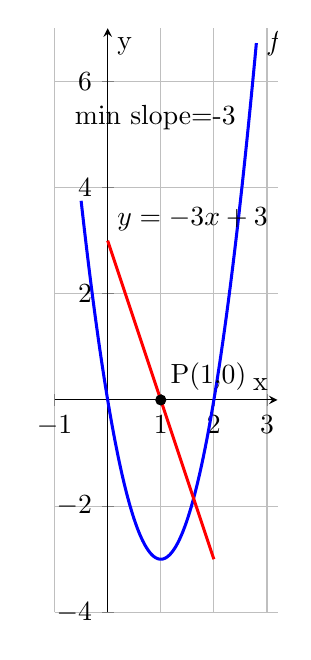
\begin{tikzpicture}
\begin{axis}[width=13cm,height=9cm,axis equal image,axis lines=middle,grid=major,xmin=-1,xmax=3.2,ymin=-4,ymax=7,xlabel={x},ylabel={y},clip=true]
\addplot[blue, solid, line width=1.1pt] coordinates {(-0.5,3.75) (-0.4725,3.504769) (-0.445,3.264075) (-0.4175,3.027919) (-0.39,2.7963) (-0.3625,2.569219) (-0.335,2.346675) (-0.3075,2.128669) (-0.28,1.9152) (-0.2525,1.706269) (-0.225,1.501875) (-0.1975,1.302019) (-0.17,1.1067) (-0.1425,0.915919) (-0.115,0.729675) (-0.0875,0.547969) (-0.06,0.3708) (-0.0325,0.198169) (-0.005,0.030075) (0.0225,-0.133481) (0.05,-0.2925) (0.0775,-0.446981) (0.105,-0.596925) (0.1325,-0.742331) (0.16,-0.8832) (0.1875,-1.019531) (0.215,-1.151325) (0.2425,-1.278581) (0.27,-1.4013) (0.2975,-1.519481) (0.325,-1.633125) (0.3525,-1.742231) (0.38,-1.8468) (0.4075,-1.946831) (0.435,-2.042325) (0.4625,-2.133281) (0.49,-2.2197) (0.5175,-2.301581) (0.545,-2.378925) (0.5725,-2.451731) (0.6,-2.52) (0.6275,-2.583731) (0.655,-2.642925) (0.6825,-2.697581) (0.71,-2.7477) (0.7375,-2.793281) (0.765,-2.834325) (0.7925,-2.870831) (0.82,-2.9028) (0.8475,-2.930231) (0.875,-2.953125) (0.9025,-2.971481) (0.93,-2.9853) (0.9575,-2.994581) (0.985,-2.999325) (1.0125,-2.999531) (1.04,-2.9952) (1.0675,-2.986331) (1.095,-2.972925) (1.1225,-2.954981) (1.15,-2.9325) (1.1775,-2.905481) (1.205,-2.873925) (1.2325,-2.837831) (1.26,-2.7972) (1.2875,-2.752031) (1.315,-2.702325) (1.3425,-2.648081) (1.37,-2.5893) (1.3975,-2.525981) (1.425,-2.458125) (1.4525,-2.385731) (1.48,-2.3088) (1.5075,-2.227331) (1.535,-2.141325) (1.5625,-2.050781) (1.59,-1.9557) (1.6175,-1.856081) (1.645,-1.751925) (1.6725,-1.643231) (1.7,-1.53) (1.7275,-1.412231) (1.755,-1.289925) (1.7825,-1.163081) (1.81,-1.0317) (1.8375,-0.895781) (1.865,-0.755325) (1.8925,-0.610331) (1.92,-0.4608) (1.9475,-0.306731) (1.975,-0.148125) (2.0025,0.015019) (2.03,0.1827) (2.0575,0.354919) (2.085,0.531675) (2.1125,0.712969) (2.14,0.8988) (2.1675,1.089169) (2.195,1.284075) (2.2225,1.483519) (2.25,1.6875) (2.2775,1.896019) (2.305,2.109075) (2.3325,2.326669) (2.36,2.5488) (2.3875,2.775469) (2.415,3.006675) (2.4425,3.242419) (2.47,3.4827) (2.4975,3.727519) (2.525,3.976875) (2.5525,4.230769) (2.58,4.4892) (2.6075,4.752169) (2.635,5.019675) (2.6625,5.291719) (2.69,5.5683) (2.7175,5.849419) (2.745,6.135075) (2.7725,6.425269) (2.8,6.72)};
\node[anchor=west] at (axis cs:2.8,6.72) {$f'(x)=3(x-1)^2-3$};
\addplot[red, solid, line width=1.1pt] coordinates {(0,3) (0.025,2.925) (0.05,2.85) (0.075,2.775) (0.1,2.7) (0.125,2.625) (0.15,2.55) (0.175,2.475) (0.2,2.4) (0.225,2.325) (0.25,2.25) (0.275,2.175) (0.3,2.1) (0.325,2.025) (0.35,1.95) (0.375,1.875) (0.4,1.8) (0.425,1.725) (0.45,1.65) (0.475,1.575) (0.5,1.5) (0.525,1.425) (0.55,1.35) (0.575,1.275) (0.6,1.2) (0.625,1.125) (0.65,1.05) (0.675,0.975) (0.7,0.9) (0.725,0.825) (0.75,0.75) (0.775,0.675) (0.8,0.6) (0.825,0.525) (0.85,0.45) (0.875,0.375) (0.9,0.3) (0.925,0.225) (0.95,0.15) (0.975,0.075) (1,0) (1.025,-0.075) (1.05,-0.15) (1.075,-0.225) (1.1,-0.3) (1.125,-0.375) (1.15,-0.45) (1.175,-0.525) (1.2,-0.6) (1.225,-0.675) (1.25,-0.75) (1.275,-0.825) (1.3,-0.9) (1.325,-0.975) (1.35,-1.05) (1.375,-1.125) (1.4,-1.2) (1.425,-1.275) (1.45,-1.35) (1.475,-1.425) (1.5,-1.5) (1.525,-1.575) (1.55,-1.65) (1.575,-1.725) (1.6,-1.8) (1.625,-1.875) (1.65,-1.95) (1.675,-2.025) (1.7,-2.1) (1.725,-2.175) (1.75,-2.25) (1.775,-2.325) (1.8,-2.4) (1.825,-2.475) (1.85,-2.55) (1.875,-2.625) (1.9,-2.7) (1.925,-2.775) (1.95,-2.85) (1.975,-2.925) (2,-3)};
\node[anchor=south west] at (axis cs:0,3) {$y=-3x+3$};
\addplot[only marks,mark=*,mark size=1.8pt,black] coordinates {(1,0)};
\node[anchor=south west] at (axis cs:1,0) {P(1,0)};
\node[anchor=south west] at (axis cs:-0.8,4.9) {min slope=-3};
\end{axis}
\end{tikzpicture}
\end{document}
